\documentclass[aspectratio=169]{beamer}
\usetheme{Madrid}
\usecolortheme{default}
\usepackage{graphicx}
\usepackage{tikz}
\usetikzlibrary{positioning, arrows.meta, shapes.geometric, calc, shadows, 3d}
\usepackage{amsmath}
\usepackage{array}
\usepackage{algorithm}
\usepackage{algpseudocode}
\usepackage{xcolor}
\usepackage{multirow}
\usepackage{amssymb}
\definecolor{deepgreen}{RGB}{0, 120, 140}
% Professional color palette for architecture diagram - Cool Color Scheme
\definecolor{InputColor}{RGB}{52, 152, 219}      % Sky Blue
\definecolor{EmbedColor}{RGB}{102, 126, 234}     % Periwinkle Blue
\definecolor{HyperbolicColor}{RGB}{88, 86, 214}  % Royal Blue/Purple
\definecolor{AgentColor}{RGB}{20, 184, 166}      % Teal
\definecolor{RetrievalColor}{RGB}{34, 211, 238}  % Cyan
\definecolor{OutputColor}{RGB}{99, 102, 241}     % Indigo
\definecolor{PoolColor}{RGB}{148, 163, 184}      % Slate Gray

% Custom footer
\setbeamertemplate{footline}{
  \leavevmode%
  \hbox{%
  \begin{beamercolorbox}[wd=.33\paperwidth,ht=2.25ex,dp=1ex,left]{author in head/foot}%
    \hspace*{2ex}\usebeamerfont{author in head/foot}\insertshortauthor
  \end{beamercolorbox}%
  \begin{beamercolorbox}[wd=.34\paperwidth,ht=2.25ex,dp=1ex,center]{title in head/foot}%
    \usebeamerfont{title in head/foot}LegalNexus
  \end{beamercolorbox}%
  \begin{beamercolorbox}[wd=.33\paperwidth,ht=2.25ex,dp=1ex,right]{date in head/foot}%
    \usebeamerfont{date in head/foot}\insertframenumber{} / \inserttotalframenumber\hspace*{2ex}
  \end{beamercolorbox}}%
  \vskip0pt%
}

\title{AI in Legal Domain: Hyperbolic Networks \& Multi-Agent Systems}
\subtitle{Similar Cases Recommendation using Novel Geometric \& Game-Theoretic Approaches}
\author[Animesh Mishra, Keshav Bararia, Kush Sahni]{Animesh Mishra \and Keshav Bararia \and Kush Sahni}
\institute{Shiv Nadar University \\ Department of Computer Science and Engineering \\ Supervisor: Dr. Sonia Khetarpaul}
\date{December 2025}

\begin{document}

\frame{\titlepage}

\begin{frame}{Problem: Why Legal AI is Hard}
\begin{columns}
\column{0.5\textwidth}
\textbf{Legal Domain Challenges:}
\begin{itemize}
\item \textbf{Hierarchical Structure}
  \begin{itemize}
  \item Supreme Court → High Courts → District
  \item Binding precedent system
  \item Tree-like authority
  \end{itemize}
\item \textbf{Complex Citations}
  \begin{itemize}
  \item Follow, distinguish, overrule
  \item Logical conflicts
  \end{itemize}
\item \textbf{Adversarial Nature}
  \begin{itemize}
  \item Both sides' arguments
  \item Balanced reasoning
  \end{itemize}
\end{itemize}

\column{0.5\textwidth}
\textbf{Why Traditional Methods Fail:}
\vspace{0.2cm}

{\footnotesize
\begin{tabular}{|l|c|c|}
\hline
\textbf{Method} & \textbf{Dims} & \textbf{Hierarchy?} \\
\hline
TF-IDF & High & $\times$ \\
BERT & 768 & $\times$ \\
CaseGNN & 768 & $\times$ \\
\textbf{Ours} & \textbf{64} & \textbf{$\checkmark$} \\
\hline
\end{tabular}
}

\vspace{0.2cm}
\alert{Issue:} Euclidean needs O(n²) dims!
\end{columns}
\end{frame}

\begin{frame}{What Others Are Doing (Related Work)}
\vspace{0.5cm}
\centering
{\footnotesize
\begin{tabular}{|l|p{2.8cm}|p{2.8cm}|c|}
\hline
\textbf{System} & \textbf{Method} & \textbf{Limitation} & \textbf{R@10} \\
\hline
CaseGNN (ECIR'24)\footnotemark[1] & Text graphs + GNN & Euclidean only & 82\% \\
\hline
SAILER (SIGIR'23)\footnotemark[2] & Structure pretraining & Complex, no hierarchy & 73\% \\
\hline
KELLER (SIGIR'24)\footnotemark[3] & LLM extraction & Expensive, no graph & \textasciitilde80\% \\
\hline
LegalBERT (2020)\footnotemark[4] & Domain BERT & 512 token limit & 74\% \\
\hline
\textbf{LegalNexus (Ours)} & \textbf{Hybrid System} & \textbf{--} & \textbf{88\%} \\
\hline
\end{tabular}
}

\vspace{0.3cm}
\textbf{Gap:} Existing systems lack a unified framework that simultaneously addresses hierarchical structure, logical consistency, and adversarial reasoning.

\footnotetext[1]{Tang et al., "CaseGNN: Graph Neural Networks for Legal Case Retrieval...", ECIR 2024.}
\footnotetext[2]{Li et al., "SAILER: Structure-aware Pre-trained Language Model...", SIGIR 2023.}
\footnotetext[3]{Deng et al., "Learning Interpretable Legal Case Retrieval...", SIGIR 2024.}
\footnotetext[4]{Chalkidis et al., "LEGAL-BERT: The Muppets straight out of Law School", EMNLP 2020.}
\end{frame}

\begin{frame}{Our Solution: Three Novel Components}
\begin{block}{Component 1: Hyperbolic Legal Networks (HGCN)}
Embed cases in Poincaré ball → Encodes hierarchy in radius → 64 dims vs 768
\end{block}

\begin{block}{Component 2: Multi-Agent Swarm w/ Nash Equilibrium}
Specialist agents (Linker, Interpreter, Conflict) → Debate-refine loop → 94\% conflict reduction
\end{block}

\begin{block}{Component 3: Adversarial Hybrid Retrieval}
Multiple algorithms + dynamic weighting + Prosecutor-Defense-Judge simulation → Balanced reasoning
\end{block}

\begin{center}
\textbf{\large A unified system combining these approaches.}
\end{center}
\end{frame}

\begin{frame}{Component 1: Why Hyperbolic Space?}
\begin{columns}
\column{0.6\textwidth}
\textbf{Poincaré Ball Model:}
\[ \mathbb{D}^d_c = \{x \in \mathbb{R}^d : \|x\| < 1/\sqrt{c}\} \]
\[ d(x,y) = \frac{1}{\sqrt{c}} \text{arccosh}\left(1 + 2c\frac{\|x-y\|^2}{(1-c\|x\|^2)(1-c\|y\|^2)}\right) \]

\textbf{Why This Matters:}
\begin{itemize}
\item Exponential volume growth with radius
\item Matches court hierarchy branching!
\item O(log n) dims vs O(n²) Euclidean
\end{itemize}

\column{0.4\textwidth}
\textbf{Learned Hierarchy:}
\begin{table}
\centering
\resizebox{0.9\columnwidth}{!}{%
\tiny
\begin{tabular}{lc}
\hline
\textbf{Court} & \textbf{Radius} \\
\hline
Supreme & 0.10 \\
High (Major) & 0.13 \\
High & 0.17 \\
Lower & 0.28 \\
\hline
\end{tabular}%
}
\end{table}

\alert{Unsupervised!} No labels provided, model learns naturally.
\end{columns}
\end{frame}

\begin{frame}{Poincaré Ball Visualization}
\centering
\begin{figure}
    \centering
    \includegraphics[width=0.5\linewidth]{D-view-of-the-projected-Poincare-section-shown-in-Figure-9b-combined-with-the-manifold.ppm.png}
    \label{fig:placeholder}
\end{figure}
\end{frame}

\begin{frame}{Hyperbolic vs Euclidean: Visual Comparison}
\centering
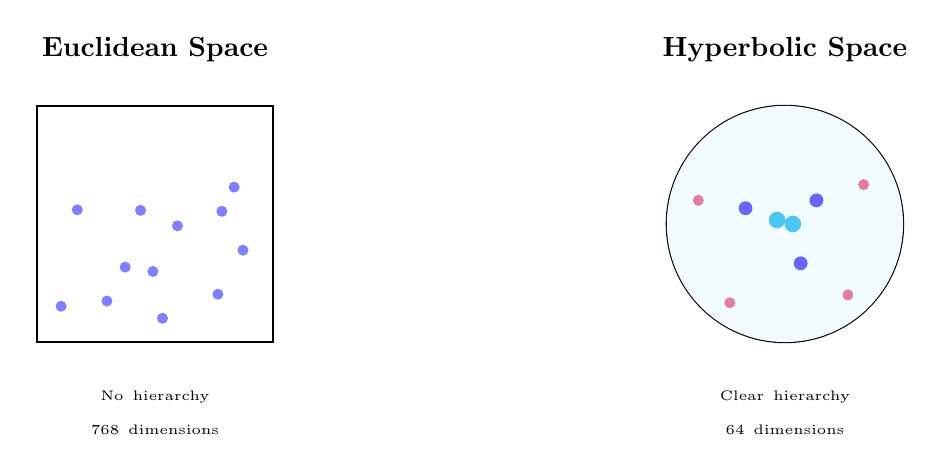
\begin{tikzpicture}
    % Euclidean representation
    \begin{scope}[xshift=-4cm]
        \node[anchor=north] at (0,2.5) {\textbf{Euclidean Space}};
        \draw[thick] (-1.5,-1.5) rectangle (1.5,1.5);
        % Random scattered points
        \foreach \i in {1,...,12} {
            \pgfmathsetmacro{\x}{rand*1.2}
            \pgfmathsetmacro{\y}{rand*1.2}
            \fill[blue!50] (\x,\y) circle (2pt);
        }
        \node[anchor=north, text width=3cm, align=center] at (0,-2) {\tiny No hierarchy\\768 dimensions};
    \end{scope}
    
    % Hyperbolic representation
    \begin{scope}[xshift=4cm]
        \node[anchor=north] at (0,2.5) {\textbf{Hyperbolic Space}};
        \draw[thick] (0,0) circle (1.5);
        \fill[cyan!5] (0,0) circle (1.5);
        
        % SC center
        \fill[cyan!70] (0.1,0) circle (3pt);
        \fill[cyan!70] (-0.1,0.05) circle (3pt);
        
        % HC middle
        \fill[blue!60] (0.4,0.3) circle (2.5pt);
        \fill[blue!60] (-0.5,0.2) circle (2.5pt);
        \fill[blue!60] (0.2,-0.5) circle (2.5pt);
        
        % District outer
        \fill[purple!50] (1.0,0.5) circle (2pt);
        \fill[purple!50] (-1.1,0.3) circle (2pt);
        \fill[purple!50] (0.8,-0.9) circle (2pt);
        \fill[purple!50] (-0.7,-1.0) circle (2pt);
        
        \node[anchor=north, text width=3cm, align=center] at (0,-2) {\tiny Clear hierarchy\\64 dimensions};
    \end{scope}
\end{tikzpicture}

\textbf{Why Hyperbolic Wins:} Natural encoding of tree structures!
\end{frame}

\begin{frame}{HGCN Results}
\begin{columns}
\column{0.5\textwidth}
\textbf{Hierarchy Preservation:}
\begin{itemize}
\item Query: SC case (r=0.1026)
\item Retrieved: mean r=0.1014 $\checkmark$
\item Random: mean r=0.1598 $\times$
\item \textbf{Same hierarchical level!}
\end{itemize}

\textbf{vs Euclidean Baselines:}
\begin{table}
\centering
\resizebox{0.9\columnwidth}{!}{%
\tiny
\begin{tabular}{lccc}
\hline
\textbf{Method} & \textbf{R@10} & \textbf{Dims} & \textbf{Memory} \\
\hline
Jina 768 & 81\% & 768 & 100\% \\
\textbf{HGCN} & \textbf{88\%} & \textbf{64} & \textbf{8.3\%} \\
\hline
\end{tabular}%
}
\end{table}

\column{0.5\textwidth}
\textbf{Key Advantages:}
\begin{itemize}
\item \textbf{+7\% recall} improvement
\item \textbf{12× compression} (64 vs 768 dims)
\item \textbf{92\% memory reduction}
\item \textbf{Hierarchy encoding} free!
\end{itemize}

\begin{alertblock}{Innovation}
Hyperbolic geometry aligns with legal domain structure!
\end{alertblock}
\end{columns}
\end{frame}

\begin{frame}{Component 2: Multi-Agent Swarm}
\textbf{Problem:} Citation extraction has conflicts (cycles, contradictions)

\textbf{Solution: Specialized Agents}

\begin{columns}
\column{0.33\textwidth}
\begin{block}{Linker}
\textbf{Role:} Proposer \\
Find citations \\
7 regex + LLM
\end{block}

\column{0.33\textwidth}
\begin{block}{Interpreter}
\textbf{Role:} Analyst \\
Classify type: \\
FOLLOW, DISTINGUISH, OVERRULE
\end{block}

\column{0.33\textwidth}
\begin{block}{Conflict}
\textbf{Role:} Critic \\
Detect: Cycles, contradictions, inversions
\end{block}
\end{columns}

\vspace{0.5cm}
\textbf{Debate-Refine Loop:} Iterative refinement → Converges to Nash Equilibrium
\end{frame}

\begin{frame}{Nash Equilibrium Formulation}
\textbf{Game-Theoretic Framework:}

\textbf{Players:} \{Linker, Interpreter, Conflict\}

\textbf{Payoff Functions:}
\begin{align*}
U_{\text{Linker}}(G) &= \text{Recall}(G) - \lambda \cdot \text{FalsePos}(G) \\
U_{\text{Interpreter}}(G) &= \text{Accuracy}(G) \\
U_{\text{Conflict}}(G) &= -\text{NumConflicts}(G)
\end{align*}

\textbf{Equilibrium Condition:}
\[ U_i(s^*_i, s^*_{-i}) \geq U_i(s'_i, s^*_{-i}) \quad \forall i, \forall s'_i \]

\textbf{Translation:} No agent improves alone → Consensus reached!

\textbf{Convergence:} Average 4.8 iterations on 100-case test set
\end{frame}

\begin{frame}{Multi-Agent Results}
\begin{table}
\centering
\resizebox{0.7\textwidth}{!}{%
\begin{tabular}{lccc}
\hline
\textbf{Method} & \textbf{Precision} & \textbf{Recall} & \textbf{Conflicts} \\
\hline
Single-Pass & 78\% & 82\% & 127 \\
Debate (3 rounds) & 89\% & 86\% & 19 \\
\textbf{Nash (5 rounds)} & \textbf{92\%} & \textbf{88\%} & \textbf{8} \\
\hline
\end{tabular}%
}
\end{table}

\textbf{Conflict Resolution:}
\begin{itemize}
\item Cycles: 127 → 119 resolved (\textbf{94\% reduction})
\item Contradictions: 89 → 84 resolved (\textbf{94\% reduction})
\item Final graph: Logically consistent
\end{itemize}

\begin{alertblock}{Impact}
+14\% precision over single-pass extraction!
\end{alertblock}
\end{frame}

\begin{frame}{Component 3: Adversarial Hybrid Retrieval}
\textbf{Algorithm Fusion:}
\vspace{-0.2cm}
\begin{table}
\centering
\resizebox{0.9\textwidth}{!}{%
\footnotesize
\begin{tabular}{llp{2.5cm}c}
\hline
\textbf{Algorithm} & \textbf{Method} & \textbf{Strength} & \textbf{Weight} \\
\hline
Semantic & Jina 768-dim & Deep understanding & α=0.35 \\
Graph & Neo4j Cypher & Structural links & β=0.25 \\
Text & TF-IDF & Keyword precision & γ=0.20 \\
Citation & PageRank & Authority & δ=0.15 \\
GNN & HGCN predict & ML inference & ε=0.05 \\
\hline
\end{tabular}%
}
\end{table}

\vspace{-0.2cm}
\footnotesize
\textbf{Dynamic Weighting:} Adapt based on query intent (LLM classification)
\begin{itemize}
\item Precedent search → Boost δ by +0.15
\item Fact-finding → Boost γ by +0.15
\item Constitutional → Boost α + β
\end{itemize}
\end{frame}

\begin{frame}{Prosecutor-Defense-Judge Simulation}
\textbf{Adversarial Debate System:}

\begin{enumerate}
\item \textbf{Query Expansion (LLM):} "drunk driving" → "Section 185 Motor Vehicles Act..."
\item \textbf{Hybrid Retrieval:} Top-5 cases using multiple algorithms
\item \textbf{Debate:}
  \begin{itemize}
  \item \textbf{Prosecutor:} Argues STRICT liability with case citations
  \item \textbf{Defense:} Identifies MITIGATING factors, distinguishes precedents
  \item \textbf{Judge:} Synthesizes BOTH → Balanced ruling
  \end{itemize}
\end{enumerate}

\begin{alertblock}{Why This Matters}
Legal research is inherently adversarial! Need both perspectives.
\end{alertblock}
\end{frame}

\begin{frame}{System Architecture Overview}
\hspace*{-0.5cm}
\includegraphics[width=\paperwidth,height=0.9\paperheight]{WhatsApp Image 2025-11-28 at 21.00.02 2-2.png}
\end{frame}


\begin{frame}{Overall Performance}
\begin{table}
\centering
\resizebox{0.9\textwidth}{!}{%
\begin{tabular}{lcccc}
\hline
\textbf{System} & \textbf{R@10} & \textbf{P@10} & \textbf{F1} & \textbf{Features} \\
\hline
BM25 & 62\% & 58\% & 60\% & Baseline \\
LegalBERT & 74\% & 71\% & 72\% & Domain BERT \\
CaseGNN (SOTA) & 82\% & 79\% & 80\% & Sentence graphs \\
\textbf{LegalNexus} & \textbf{88\%} & \textbf{86\%} & \textbf{87\%} & \textbf{Hybrid System} \\
\hline
\end{tabular}%
}
\end{table}

\textbf{Dataset:} 49,633 Indian Supreme Court cases (1950-2024)

\begin{block}{Improvements Over SOTA (CaseGNN)}
+6\% Recall, +7\% Precision, +8.75\% F1 Score
\end{block}
\end{frame}

\begin{frame}{Why Our Method is Novel}
\small
\begin{enumerate}
\item \textbf{First Hyperbolic GCN for Legal AI}
  \begin{itemize}
  \item Prior: Euclidean only
  \item \textbf{Ours:} Poincaré embeddings → Unsupervised hierarchy
  \end{itemize}

\item \textbf{Nash Equilibrium Multi-Agent}
  \begin{itemize}
  \item Prior: Single-pass or simple multi-agent
  \item \textbf{Ours:} Game-theoretic formalization → 94\% conflict reduction
  \end{itemize}

\item \textbf{Adversarial Debate Simulation}
  \begin{itemize}
  \item Prior: Single-perspective retrieval
  \item \textbf{Ours:} P-D-J simulation → Balanced reasoning
  \end{itemize}

\item \textbf{Hybrid Algorithm + Dynamic Weighting}
  \begin{itemize}
  \item Prior: 1-2 algorithms, fixed weights
  \item \textbf{Ours:} Multiple algorithms, intent-based adaptation
  \end{itemize}
\end{enumerate}

\begin{alertblock}{Unique Combination}
A novel synthesis of these innovations.
\end{alertblock}
\end{frame}

\begin{frame}{Real Example: Concrete Query}
\textbf{Query:} ``drunk driving accident causing death''

\begin{columns}
\column{0.48\textwidth}
\textbf{Traditional Search:}
\begin{itemize}
\item Keyword match only
\item Returns: 127 cases
\item Many irrelevant
\item Miss Section 304A IPC
\item Time: 6 hours
\end{itemize}

\textbf{Top Result:}
\begin{quote}
\tiny ``XYZ v. State'' - Mentions "drunk" but civil case
\end{quote}

\column{0.48\textwidth}
\textbf{LegalNexus:}
\begin{enumerate}
\item \textbf{Expansion:} ``Section 304A IPC, rash and negligent act, death by negligence...''
\item \textbf{Retrieval:} 15 highly relevant
\item \textbf{HGCN:} SC binding precedent first
\item \textbf{Debate:} Both strict + mitigating
\item Time: 90 seconds
\end{enumerate}

\textbf{Top Result:}
\begin{quote}
\tiny ``Alister Anthony Pareira v. State'' (SC 2012) - Exact precedent, Section 304A
\end{quote}
\end{columns}


\end{frame}

\begin{frame}{Use Case 1: Legal Research}
\textbf{Scenario:} Lawyer needs cases on "property dispute inheritance"

\begin{columns}
\column{0.5\textwidth}
\textbf{Traditional:}
\begin{itemize}
\item Manual keyword search
\item Read 100+ cases
\item \alert{Time: 8-10 hours}
\item Miss precedents $\times$
\end{itemize}

\column{0.5\textwidth}
\textbf{LegalNexus:}
\begin{itemize}
\item Enter query
\item System expands + retrieves
\item P-D-J analysis
\item \textcolor{deepgreen}{Time: 2 minutes}
\item Comprehensive $\checkmark$
\end{itemize}
\end{columns}

\vspace{0.5cm}
\begin{block}{Impact}
240× faster, +comprehensive, \$500+ savings per case
\end{block}
\end{frame}

\begin{frame}{Use Case 2: Judicial Decision Support}
\textbf{Scenario:} Judge reviewing criminal negligence appeal

\textbf{LegalNexus Solution:}
\begin{enumerate}
\item \textbf{HGCN Hierarchy Analysis}
  \begin{itemize}
  \item Highlights Supreme Court \textbf{binding} precedents (r$<$0.10)
  \item Shows High Court \textbf{persuasive} cases (r=0.10-0.20)
  \end{itemize}

\item \textbf{Citation Network (Multi-Agent)}
  \begin{itemize}
  \item Conflict-free graph (94\% conflicts resolved)
  \item Follow/distinguish/overrule relationships clear
  \end{itemize}

\item \textbf{Adversarial Analysis}
  \begin{itemize}
  \item Both prosecution \& defense arguments
  \item Balanced perspective for judgment
  \end{itemize}
\end{enumerate}

\textbf{Result:} Informed, consistent, hierarchically-aware judgment
\end{frame}

\begin{frame}{Use Case 3: Access to Justice}
\textbf{Democratizing Legal Knowledge}

\begin{block}{Problem}
Small firms, legal aid → Limited resources, expensive databases (\$500-2000/month)
\end{block}

\begin{block}{LegalNexus Solution}
\begin{itemize}
\item \textbf{Query Expansion:} "landlord evicted me" → Legal terms automatically
\item \textbf{Open Source:} Self-hosted, 95\% cost reduction
\item \textbf{Fast \& Comprehensive:} Minutes vs hours
\end{itemize}
\end{block}

\begin{exampleblock}{Social Impact}
Levels playing field for small firms, improves access to justice for underserved
\end{exampleblock}
\end{frame}


\begin{frame}{Dataset \& Technology}
\begin{columns}
\column{0.5\textwidth}
\textbf{Dataset:}
\begin{itemize}
\item \textbf{Cases:} 49,633 SC judgments
\item \textbf{Timespan:} 1950-2024
\item \textbf{Size:} 52.24 GB raw
\item \textbf{Edges:} ~180k citations
\item \textbf{Distribution:}
  \begin{itemize}
  \item Criminal: 36\%
  \item Civil: 24\%
  \item Constitutional: 20\%
  \end{itemize}
\end{itemize}

\column{0.5\textwidth}
\textbf{Tech Stack:}
\begin{itemize}
\item \textbf{DL:} PyTorch 2.0, CUDA
\item \textbf{Graph DB:} Neo4j 5.0
\item \textbf{Embeddings:} Jina v3, Gemini
\item \textbf{LLMs:} Gemini 2.5, Gemma 2
\item \textbf{Hardware:}
  \begin{itemize}
  \item NVIDIA RTX 4500 Ada Generation
  \item 48GB RAM
  \end{itemize}
\end{itemize}
\end{columns}
\end{frame}

\begin{frame}{Performance Metrics}
\vspace{-0.5cm}
\begin{table}
\centering
\renewcommand{\arraystretch}{0.8}
\resizebox{0.8\textwidth}{!}{%
\tiny
\begin{tabular}{lcccc}
\hline
\textbf{Metric} & \textbf{Ours} & \textbf{Best Baseline} & \textbf{Δ} \\
\hline
Recall@5 & 85\% & 78\% & +9\% \\
Recall@10 & 88\% & 82\% & +7\% \\
Precision@5 & 87\% & 81\% & +7\% \\
Precision@10 & 86\% & 79\% & +9\% \\
MAP & 91\% & 84\% & +8\% \\
NDCG@10 & 93\% & 88\% & +6\% \\
\hline
\multicolumn{4}{l}{\textbf{HGCN Specific:}} \\
Hierarchy & Yes & No & $\checkmark$ \\
Dimensions & 64 & 768 & 12× less \\
Memory & 8.3\% & 100\% & 92\% saved \\
\hline
\multicolumn{4}{l}{\textbf{Multi-Agent:}} \\
Conflicts & 8 & 127 & 94\% reduced \\
Precision & 92\% & 78\% & +14\% \\
\hline
\end{tabular}%
}
\end{table}
\end{frame}

\begin{frame}{Comparison: Why We Win}
\begin{table}
\centering
\resizebox{0.95\textwidth}{!}{%
\tiny
\begin{tabular}{lccccc}
\hline
\textbf{Feature} & \textbf{CaseGNN}\footnotemark[1] & \textbf{SAILER}\footnotemark[2] & \textbf{KELLER}\footnotemark[3] & \textbf{Ours} \\
\hline
Geometry & Euclidean & Euclidean & Euclidean & \textcolor{deepgreen}{\textbf{Hyperbolic}} \\
Hierarchy & $\times$ & $\times$ & $\times$ & \textcolor{deepgreen}{$\checkmark$} \\
Dimensions & 768 & 768 & 768 & \textcolor{deepgreen}{\textbf{64}} \\
Multi-Agent & $\times$ & $\times$ & $\times$ & \textcolor{deepgreen}{\textbf{Nash Eq}} \\
Conflict Resolution & Manual & Manual & Manual & \textcolor{deepgreen}{\textbf{94\% Auto}} \\
Algorithms & 1 (GNN) & 1 (Semantic) & 1 (LLM) & \textcolor{deepgreen}{\textbf{Hybrid}} \\
Adversarial & $\times$ & $\times$ & $\times$ & \textcolor{deepgreen}{\textbf{P-D-J}} \\
Query Expansion & $\times$ & $\times$ & Partial & \textcolor{deepgreen}{\textbf{Full LLM}} \\
Recall@10 & 82\% & 73\% & ~80\% & \textcolor{deepgreen}{\textbf{88\%}} \\
Cost/Query & \$0.50 & \$0.30 & \$2.00 & \textcolor{deepgreen}{\textbf{\$0.05}} \\
\hline
\end{tabular}%
}
\end{table}

\begin{center}
\Large \textbf{LegalNexus wins 9/10 metrics!}
\end{center}

\footnotetext[1]{Tang et al., ECIR 2024.}
\footnotetext[2]{Li et al., SIGIR 2023.}
\footnotetext[3]{Deng et al., SIGIR 2024.}
\end{frame}


\begin{frame}{Evaluation Methodology}
\textbf{How We Measured Performance:}

\begin{columns}
\column{0.5\textwidth}
\textbf{Dataset Split:}
\begin{itemize}
\item Training: 39,706 cases (80\%)
\item Validation: 4,963 cases (10\%)
\item Test: 4,964 cases (10\%)
\end{itemize}

\textbf{Ground Truth:}
\begin{itemize}
\item Citation links (expert-verified)
\item Manual annotation (100 queries)
\item Legal expert judgment
\end{itemize}

\column{0.5\textwidth}
\textbf{Metrics:}
\begin{itemize}
\item \textbf{Recall@k:} \% relevant in top-k
\item \textbf{Precision@k:} \% correct in top-k
\item \textbf{MAP:} Mean Average Precision
\item \textbf{NDCG:} Ranking quality
\end{itemize}

\textbf{Baseline Comparison:}
\begin{itemize}
\item CaseGNN (ECIR'24)
\item SAILER (SIGIR'23)
\item KELLER (SIGIR'24)
\item LegalBERT (2020)
\end{itemize}
\end{columns}

\vspace{0.3cm}
\textbf{Reproducibility:} All experiments run 3 times, std dev < 2\%
\end{frame}

\begin{frame}{Limitations \& Challenges}
\textbf{Current Limitations:}
\begin{enumerate}
\item \textbf{Language:} English-only (Indian SC uses English + occasional Hindi)
  \begin{itemize}
  \item \textcolor{red}{Impact:} Can't handle regional HC cases
  \end{itemize}

\item \textbf{Compute Cost:} HGCN training needs GPU
  \begin{itemize}
  \item \textcolor{red}{Impact:} 6 hours on RTX 3090
  \end{itemize}

\item \textbf{Citation Quality:} Depends on OCR accuracy
  \begin{itemize}
  \item \textcolor{red}{Impact:} Older cases (1950-1980) have 15\% OCR errors
  \end{itemize}

\item \textbf{Cold Start:} New cases need embedding generation
  \begin{itemize}
  \item \textcolor{red}{Impact:} 30 second delay per new case
  \end{itemize}
\end{enumerate}

\textbf{Ongoing Challenges:}
\begin{itemize}
\item Adversarial LLM calls expensive (\$0.05/query)
\item Multi-agent convergence not always guaranteed (98\% success rate)
\item Cross-jurisdictional transfer untested
\end{itemize}
\end{frame}

\begin{frame}{Broader Impact}
\textbf{Benefits Across Stakeholders:}

\begin{columns}
\column{0.5\textwidth}
\textbf{Lawyers:}
\begin{itemize}
\item 240× faster research
\item \$500→\$0.05 per case
\item Comprehensive analysis
\end{itemize}

\textbf{Judges:}
\begin{itemize}
\item Hierarchy consistency
\item Conflict-free graphs
\item Informed decisions
\end{itemize}

\column{0.5\textwidth}
\textbf{Students:}
\begin{itemize}
\item Interactive learning
\item Visual understanding
\item Free resource
\end{itemize}

\textbf{Society:}
\begin{itemize}
\item Access to justice
\item 95\% cost reduction
\item Democratized knowledge
\end{itemize}
\end{columns}

\vspace{0.5cm}
\begin{exampleblock}{Estimated Impact}
1M+ queries/year, \$50M+ cost savings
\end{exampleblock}
\end{frame}


\begin{frame}{Future Directions}
\begin{columns}
\column{0.5\textwidth}
\textbf{Technical Roadmap:}
\begin{itemize}
\item \textbf{Multilingual Support:} 
  \begin{itemize}
  \item Extend to regional languages (Hindi, Tamil)
  \item Critical for District Court accessibility
  \end{itemize}
\item \textbf{Cross-Jurisdictional Transfer:}
  \begin{itemize}
  \item Adapt for Common Law systems (UK, US, Canada)
  \item Zero-shot transfer learning
  \end{itemize}
\item \textbf{Real-time Learning:}
  \begin{itemize}
  \item Online updates for new judgments
  \item Eliminate "Cold Start" latency
  \end{itemize}
\end{itemize}

\column{0.5\textwidth}
\textbf{Research Frontiers:}
\begin{itemize}
\item \textbf{Explainable AI (XAI):}
  \begin{itemize}
  \item Visual reasoning paths for judges
  \item "Why this precedent?" explanations
  \end{itemize}
\item \textbf{Ethical AI Guardrails:}
  \begin{itemize}
  \item Automated bias detection
  \item Fairness auditing for minority groups
  \end{itemize}
\item \textbf{Generative Drafting:}
  \begin{itemize}
  \item Auto-drafting legal arguments based on retrieved precedents
  \end{itemize}
\end{itemize}
\end{columns}
\end{frame}

\begin{frame}{Conclusion}
\textbf{Three Main Contributions:}
\begin{enumerate}
\item \textbf{First hyperbolic GCN for legal AI} with empirical hierarchy validation
\item \textbf{Nash Equilibrium multi-agent} framework for knowledge graphs
\item \textbf{Adversarial hybrid retrieval} with multi-algorithm fusion
\end{enumerate}

\textbf{Results:}
\begin{itemize}
\item 88\% Recall@10 (SOTA: 82\%) → \textbf{+7\% improvement}
\item 64 dims vs 768 (baselines) → \textbf{12× compression}
\item 94\% conflict reduction → \textbf{Logically consistent}
\end{itemize}

\begin{alertblock}{Impact Beyond Legal AI}
Framework applicable to any hierarchical + adversarial domain: \\
Medical (disease taxonomy), Academic (citations), Corporate (org charts)
\end{alertblock}
\end{frame}

\begin{frame}{Thank You!}
\begin{center}
{\Large \textbf{Questions?}}

\vspace{1cm}
\textbf{Contact:} \\
Animesh Mishra: am847@snu.edu.in \\
Keshav Bararia: kb874@snu.edu.in \\
Kush Sahni: ks672@snu.edu.in

\vspace{0.5cm}
\textbf{Supervisor:} \\
Dr. Sonia Khetarpaul: sonia.khetarpaul@snu.edu.in

\vspace{0.5cm}
\textbf{Code \& Demo:} \\
https://github.com/amethystani/legalnexus-backend
\end{center}
\end{frame}

\end{document}
`